\documentclass[12pt]{article}
\usepackage{graphicx}
\usepackage[section]{placeins}
\usepackage{amsmath}
\usepackage{enumitem}
\usepackage{tcolorbox}
\usepackage{subfigure}
\usepackage{amssymb}
\usepackage{hyperref}

\title{Controlled Procedural Terrain Generation}
\author{Alfredo Russo}
\date{A.A. 2021-2022}

\begin{document}
    \maketitle
    \newpage
    \tableofcontents
    \newpage
    

    \section{Introduction}

    \section{Coastline Agent}

    \section{Smoothing Agent}
    Smoothing agent is the one which deals with smoothing points previously elevated by the coastline agent.
    In order to do that it use extended Von Neumann neighbourhood, changing the height of the points while it perform a random walk 
    on the map.
    
    \subsection{Agent parameter}
    Like every agent it has parameters that allow designer to led different results based on it.
    These parameters are:
    \begin{itemize}
        \item \textbf{AgentNr:} it represents the number of agent that will be placed on the map in order to smooth coastline points.
        \item \textbf{returnValue:} this is a value used for understand when the agent have to came back to its starting point. The more the value is high, the more
        the points near the starting point will be smooth. So the agent came back to the starting point periodically and this is useful if some parts of the map need 
        more smoothing than others.
        \item \textbf{smoothingTokens:} it represents, like all other agent, the number of action that the agent can perform. The more the number is high, the more the map will be smooth.
    \end{itemize}

    For speeding up the computation there is another parameters taken by the coastline agent script which is \textbf{coastline points}, so the points where it is possible to place agents.
    This is done because retrieving coastline points (points which height is more than 0) can be perforamce expensive depending on how much the map is big. 

    \noindent 
    Smoothing agent require terrain to work, so there are all the parameters related to the terrain like \textbf{terrain data}, \textbf{heightmap} and so on \dots

    \noindent
    There is also a parameter called \textbf{neighboringPoint} which is used when the agent have to move itself in an adjacent point.
    
    \noindent
    At the end there is an instance of the smoothing agent in order to let the agent start working after and only after the coastline agent finish its work.

    \subsection{Action}
    This method represents the agent action on the map, but before it can start there are a couple of thing to do.
    The first thing is to retrieve all the heights related to map points previously generated by the coastline agent. So the heighmap matrix is filled with this information.
    The second one is to retrieve all the coastline point (the point with heights greater than 0) in order to place the agents on the map. This is done by retrieving the
    related hashset by the coastline agent script in order to avoid useless computation. Furthermore the complexity of this kind of computation increase with the map size 
    because it is nedeed to check every point height of the map.
    After these things the action can start.

    Every agent need to be placed on the map but not in a completely random way. The agents have to be placed on a coastline point, so in order to do that a random point is retrieve
    from the haseset which contains them and assigned to the starting point. This point is very important for the smoothing agent because, as previously said, this agent returns
    to its starting point periodically.

    In order to understand when the agent have to return to its starting point it is used a counter (\textbf{count}) originally set to 0;
    
    It is important to track the position of every agent and for this is used a variable called \textbf{location} that it is updated during time with the current agent postion. 
    At the beggining it is set to the value of the starting point.

    Every agent can perform an action according with the number of the tokens specified. The action can consist of came back to the starting point or change the height of a point
    with extended VonNeumannNeighborood.

    If the value specified as \textbf{returnValue} is 5, it means that the agent have to came back to the starting point 5 times. In order to compute after how many action the agent
    have to came back, the number of tokens is divided by the returnValue. So if the counter is greater than this value the agent have to came back, the location is set to the
    starting point and the counter is set to 0. Otherwise the agent can perform its action computing the new height for the point where it is and then update the value in the haightmap.
    After this, the agent move itself on a valid random neighboring point thanks to the \textbf{GetNeighboringPoint} method and the counter is incresed by one.

    I choose to use unity coroutine, so every time an agent end its work, the terrain is updated with the new heighmap values.

    \subsection{VonNeumannNeighborood} \label{section:Von Neumann}
    The VonNeumannNeighborood method compute the new height of the given point p as the average of points in an extended von Neumann neighborhood of p consisting of the
    four orthogonal map points surrounding p on the elevation grid and the four points beyond these, see figure \ref{fig:vonNeumann}.

    \begin{figure}
        \centering
        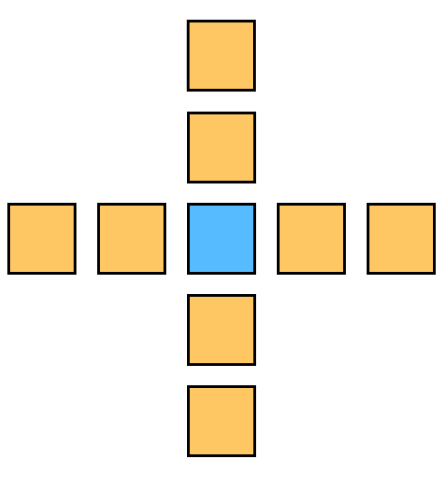
\includegraphics[scale = 0.7]{images/Extended VonNeumannNeighborhood.png}
        \caption{Extended Von Neumann Neighborood}
        \label{fig:vonNeumann}
    \end{figure}

    \noindent
    A weighted average height is calculated, with the center point given 3 times the weight of the other points. Therefore nine points with a total weight of eleven are used.
    Starting from this information it is possible to calculate the weight for the central point and the weight for the surrounding points resolving the following equation system:

    \begin{equation}
        \begin{cases}
            x + y = 11
            \\ 3x = y
        \end{cases}
    \end{equation}

    \noindent
    The variable x represents the weight for the central point which is 3 times the other points weight represented by y. So the central point weight is 11/4 and other points weight is 33/4.

    Then the heights of all the points are collected, but it can happen that a surrounding point of location is outside the map. In this case the height considered  is the location one. 
    This choice is done because otherwise the more the points are near to the end of the map, the more their heights will be near to zero, see figure \ref{fig:SmotthingCamparison}.
    
    \begin{figure}
        \centering     %%% not \center
        \subfigure[Height = 0]{\label{fig:Height0}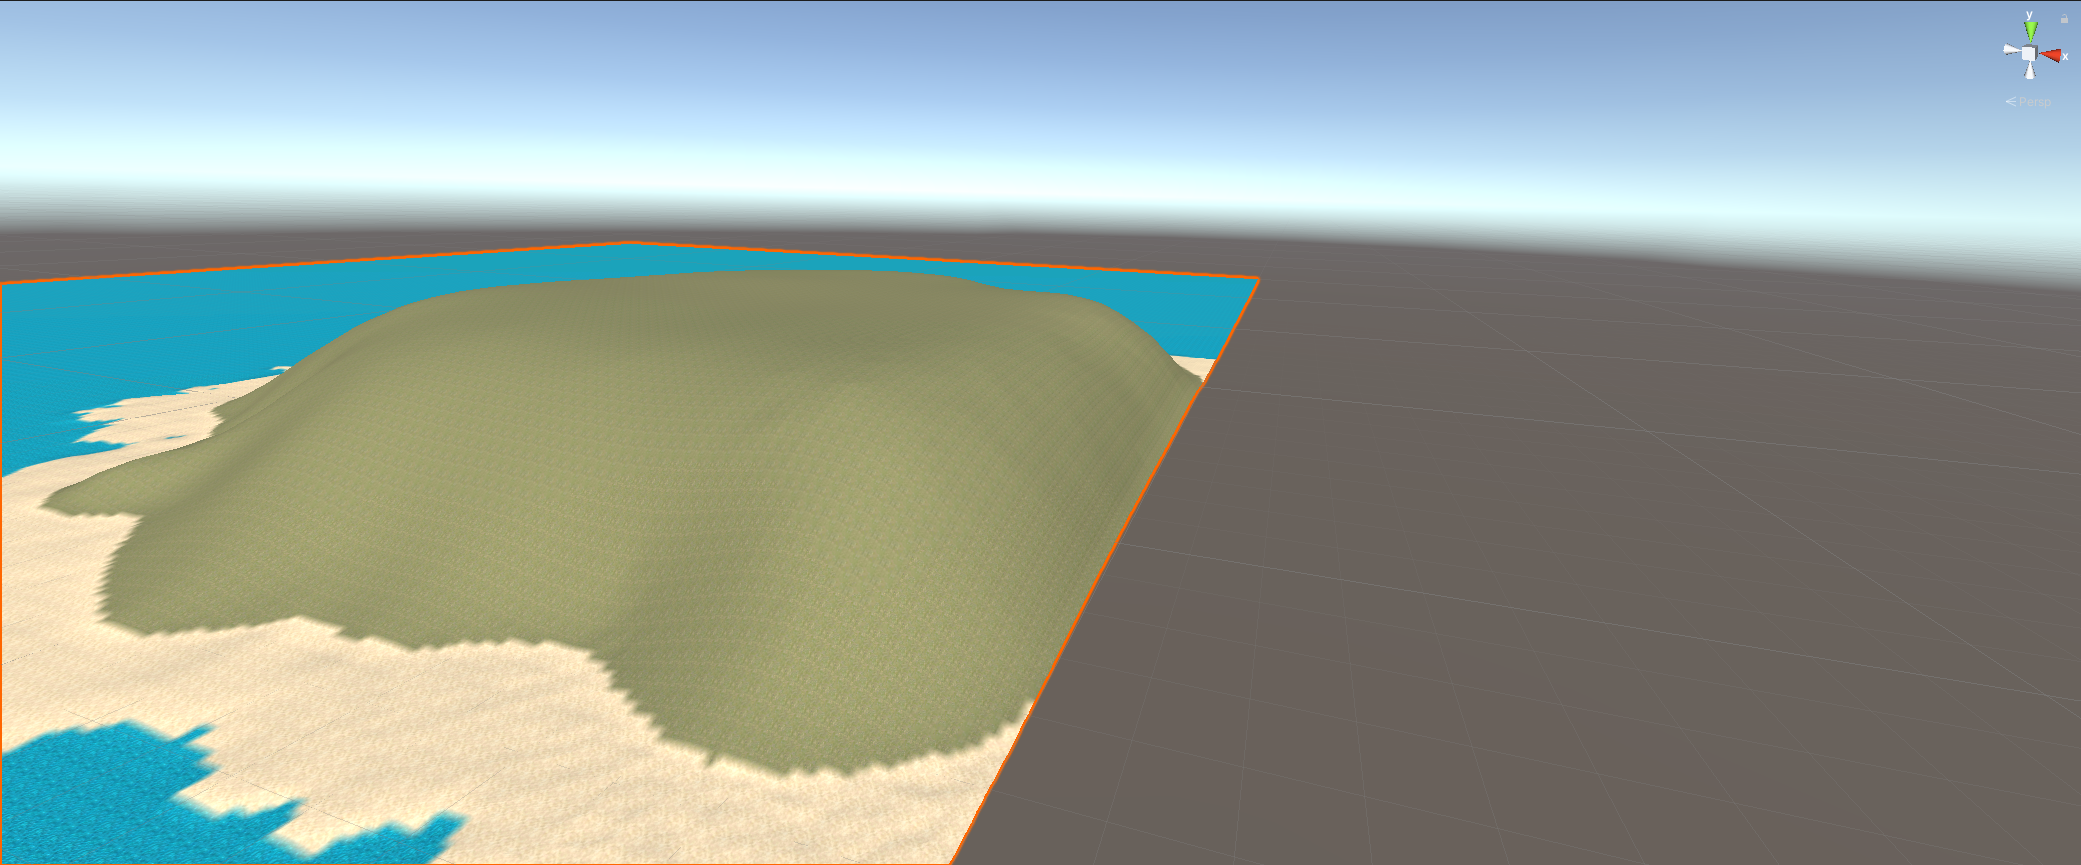
\includegraphics[width=60mm]{images/Smoothing agent height 0}}
        \subfigure[Height = location height]{\label{fig:LocationHeight}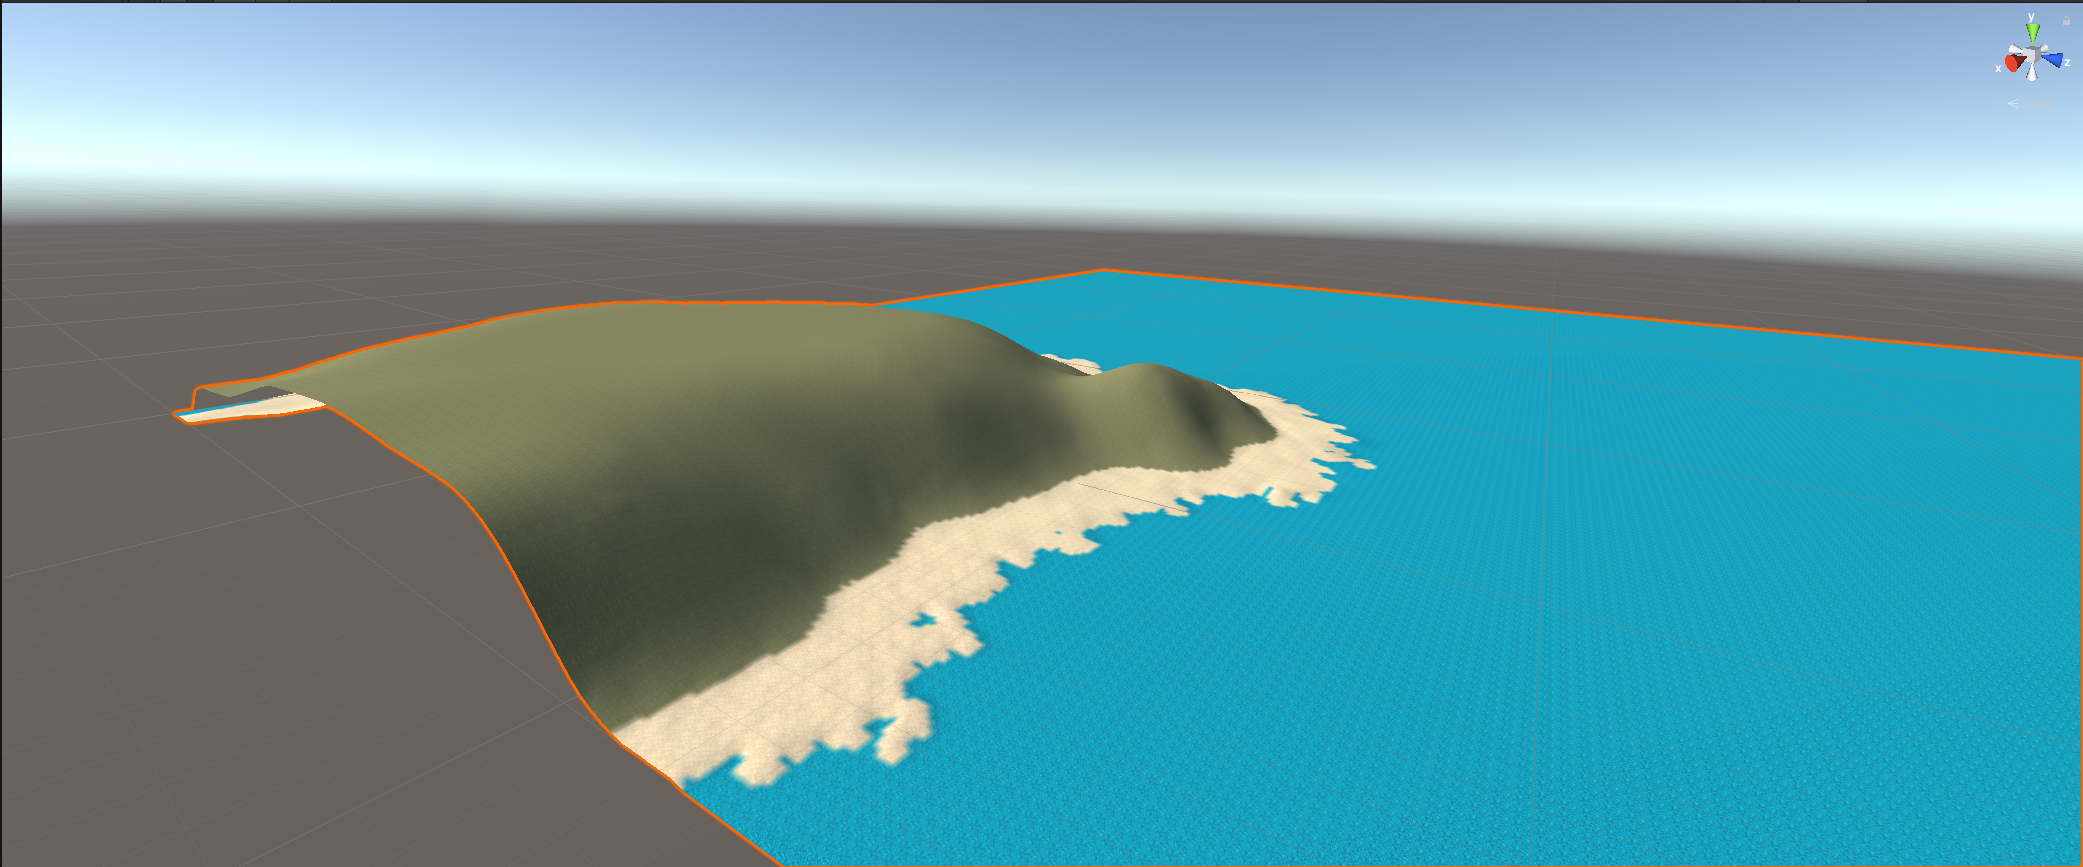
\includegraphics[width=60mm]{images/Smoothing agent height location}}
        \caption{Two different smoothing results.}
        \label{fig:SmotthingCamparison}
    \end{figure}
        
    
    After collected all heights the weighted average height is calculated as follow:

    \begin{equation}
        a = \dfrac{\sum\limits_{i=0}^{9} (W_i * H_i) }{ \sum\limits_{i=0}^{9} W_i }
    \end{equation}

    \noindent
    Where W represent the weight and H represent the height value related to the point. 

    \subsection{GetNeighboringPoint}
    This method takes the current location of the agent and starting from this check if the neighboring point are inside the terrain and then add it to a list. After it is choosen a 
    random point between the valid ones found.

    In order to check if a point is inside the terrain it is used the method called \textbf{IsInsideTerrain} that check if the coordinate of the point are between the range 0 and
    the limit of the map.

    \section{Beach Agent}
    This agent start its work after smoothing agent ends its own. In order to do that it is used an instancce of the agent that allow to start the action after smoothing agent end its work.
    Beach agent has the work to generate beach according with the parameter choosen by the designer.
    According to this it is possible to obtain a very huge beach all around the coastline or small one in some part of it. It is also possible
    to have flat beach or one that allow fluctuation in its height.

    \subsection{Agent Parameter}
    The beach agent have the following parameter that designer can exploit to generate a different kind of beach:

    \begin{itemize}
        \item \textbf{beachAgentNr:} it represents the number of agent that will work for generating beach.
        \item \textbf{beachTokens:} it is the number of action that each agent have.
        \item \textbf{heightLimit:} it is the altidue limit, when the agent reach a point higher than the limit specified, it leave the area
        and move to another random shoreline point.
        \item \textbf{randomWalkSize:} when the agent is placed on a random shoreline point it jump away from it changing the height of
        the point and smoothing them according to the parameters specified. How long will be its walk is specified by randomWalkSize parameter.
        \item \textbf{awayLimit:} when the agent have to jump away from the coastline it is needed to know how much far the agent have to jump away.
        So the awayLimit parameter it is really important since it specify that information.
        \item \textbf{beachHeight:} it is a range between [0.003, 0.01[ that represent beach height. Actually, in Unity, we are woking with heightmap
        matrix where the heights are mapped inside the range 0-1. So the value previously written have to be multiplied by the maximum height of the 
        unity terrain. If the maximum height of the unity terrain is 100, the range previously specified becomes [0.3, 1[.
    \end{itemize}

    \subsection{Action}
    Before starting beach agent action, the heightmap matrix have to be filled with the value related to the points height of unity terrain.
    
    \noindent
    After the smoothing agent action, it can heppen that there are points with height between 0 and 0.003 which are neither sea point nor beach point. In 
    order to avoid this behaviour a method called \textbf{FlatPoints} is invoked. This method set the height of those points to 0.
    In order to place the agent on the map and replace it when the agent get stuck, a list with all the shoreline points is used and filled thanks to \textbf{GetShorelinePoints}
    method.
    
    Every agent have to be placed on the map, so at the beginning it is retrieved a random shoreline point from the list previously mentioned and the value is assigned to location
    which represents the current position of the agent that will change over time.

    After the agent is placed on the map it can start its work. The first things to do is to check if the location has an height value greater than the \textbf{heightLimit}.
    If it is, the agent have to be replaced on the map and its location is changed to another random shoreline point.
    
    Then location point and the points around it are flatten and this means that a random height value between the \textbf{beachHeight} range is assigned
    to them. After these points are smoothed using Von Neumann Neighborood, see section \ref{section:Von Neumann}.

    Then the agent move itself to a random point away from the coast using \textbf{AwayRandomPoint} method. The new point is stored inside a different variable
    than location since after the agent ends its random walk, it have to came back to the location and move itself to another shoreline point near location.

    Now the agent is ready to start its random walk which duration depends on the parameter \textbf{randomWalkSize}. The agent start to faltten and smooth the away point
    and its neighboring point and only after it moves itself to a valid neighboring point exploiting \textbf{GetNeighboringPoint} method. A point is a valid one if it is 
    inside the map and its height is less than 0.01. It is possible that no valid point near the current position of the agent is found, if it happens means that the 
    agent isn't able to move itself to another point, so its random walk ends. For checking this, it is used a placeholder parameter which is the value Vector2Int.one.

    When the agent random walk ends the agent move itself to a new shoreline point near the shoreline point where it was before, assigning the new value to the 
    location variable.

    \subsection{CheckShorelinePoint}
    This method is used by \textbf{GetShorelinePoints} one in order to check if a point is a shoreline one or not. It return true if the point has an height value
    between the range [0.003, 0.01[. This range was choosen so the points retrieved are point quite close to the sea. Another thing to check by this method is
    if the coordinate of the point plus the away limit are inside the map or not, in order to understand if the agent starting from this point is able to jump away from it.

    \subsection{GetNeighboringPoint}
    This method is used in order to retrieve a position where the agent can move itself exploiting \textbf{GetNeighboringPoints} method which return all
    valid points. If there aren't no valid points around the location a placeholder value is returned in order to communicate that the agent isn't able
    to move itself.

    \subsection{AwayRandomPoint}
    As previously said, this method allow the agent to jump away from the coast. It add to location a direction multiplied by the \textbf{awayLimit} in order
    to retrieve a point away from the coast and check if it is inside the terrain and its height is less than 0.01. It will be for sure a point away starting
    from the one given in input because every shoreline point can be called like this only if it allow to jump away from it. This check is done by 
    \textbf{GetShorelinePoints} method.

    \section{City Agent}

    \section{Tree Agent}
 
    \section{Harbor Agent}

\end{document}